\documentclass{sigchi}

% Arabic page numbers for submission. 
% Remove this line to eliminate page numbers for the camera ready copy
\pagenumbering{arabic}

\usepackage{cite}
\usepackage{balance}  % to better equalize the last page
\usepackage{graphics} % for EPS, load graphicx instead
\usepackage{times}    % comment if you want LaTeX's default font
\usepackage{url}      % llt: nicely formatted URLs
\usepackage{color}
\usepackage{pdfpages}

%\usepackage[version=4]{mhchem}
\newcommand*\ce[1]{\ensuremath{\mathrm{#1}}}


\makeatletter
\def\url@leostyle{%
  \@ifundefined{selectfont}{\def\UrlFont{\sf}}{\def\UrlFont{\small\bf\ttfamily}}}
\makeatother
\urlstyle{leo}

\def\pprw{8.5in}
\def\pprh{11in}
\special{papersize=\pprw,\pprh}
\setlength{\paperwidth}{\pprw}
\setlength{\paperheight}{\pprh}
\setlength{\pdfpagewidth}{\pprw}
\setlength{\pdfpageheight}{\pprh}

% Make sure hyperref comes last of your loaded packages, 
% to give it a fighting chance of not being over-written, 
% since its job is to redefine many LaTeX commands.
\usepackage[pdftex]{hyperref}
\hypersetup{
pdftitle={report},
pdfauthor={LaTeX},
pdfkeywords={SIGCHI, proceedings, archival format},
bookmarksnumbered,
pdfstartview={FitH},
colorlinks,
citecolor=black,
filecolor=black,
linkcolor=black,
urlcolor=black,
breaklinks=true,
}

\newcommand\tabhead[1]{\small\textbf{#1}}
\newcommand\todo[1]{\textcolor{red}{#1}}


\begin{document}
\pagenumbering{gobble}
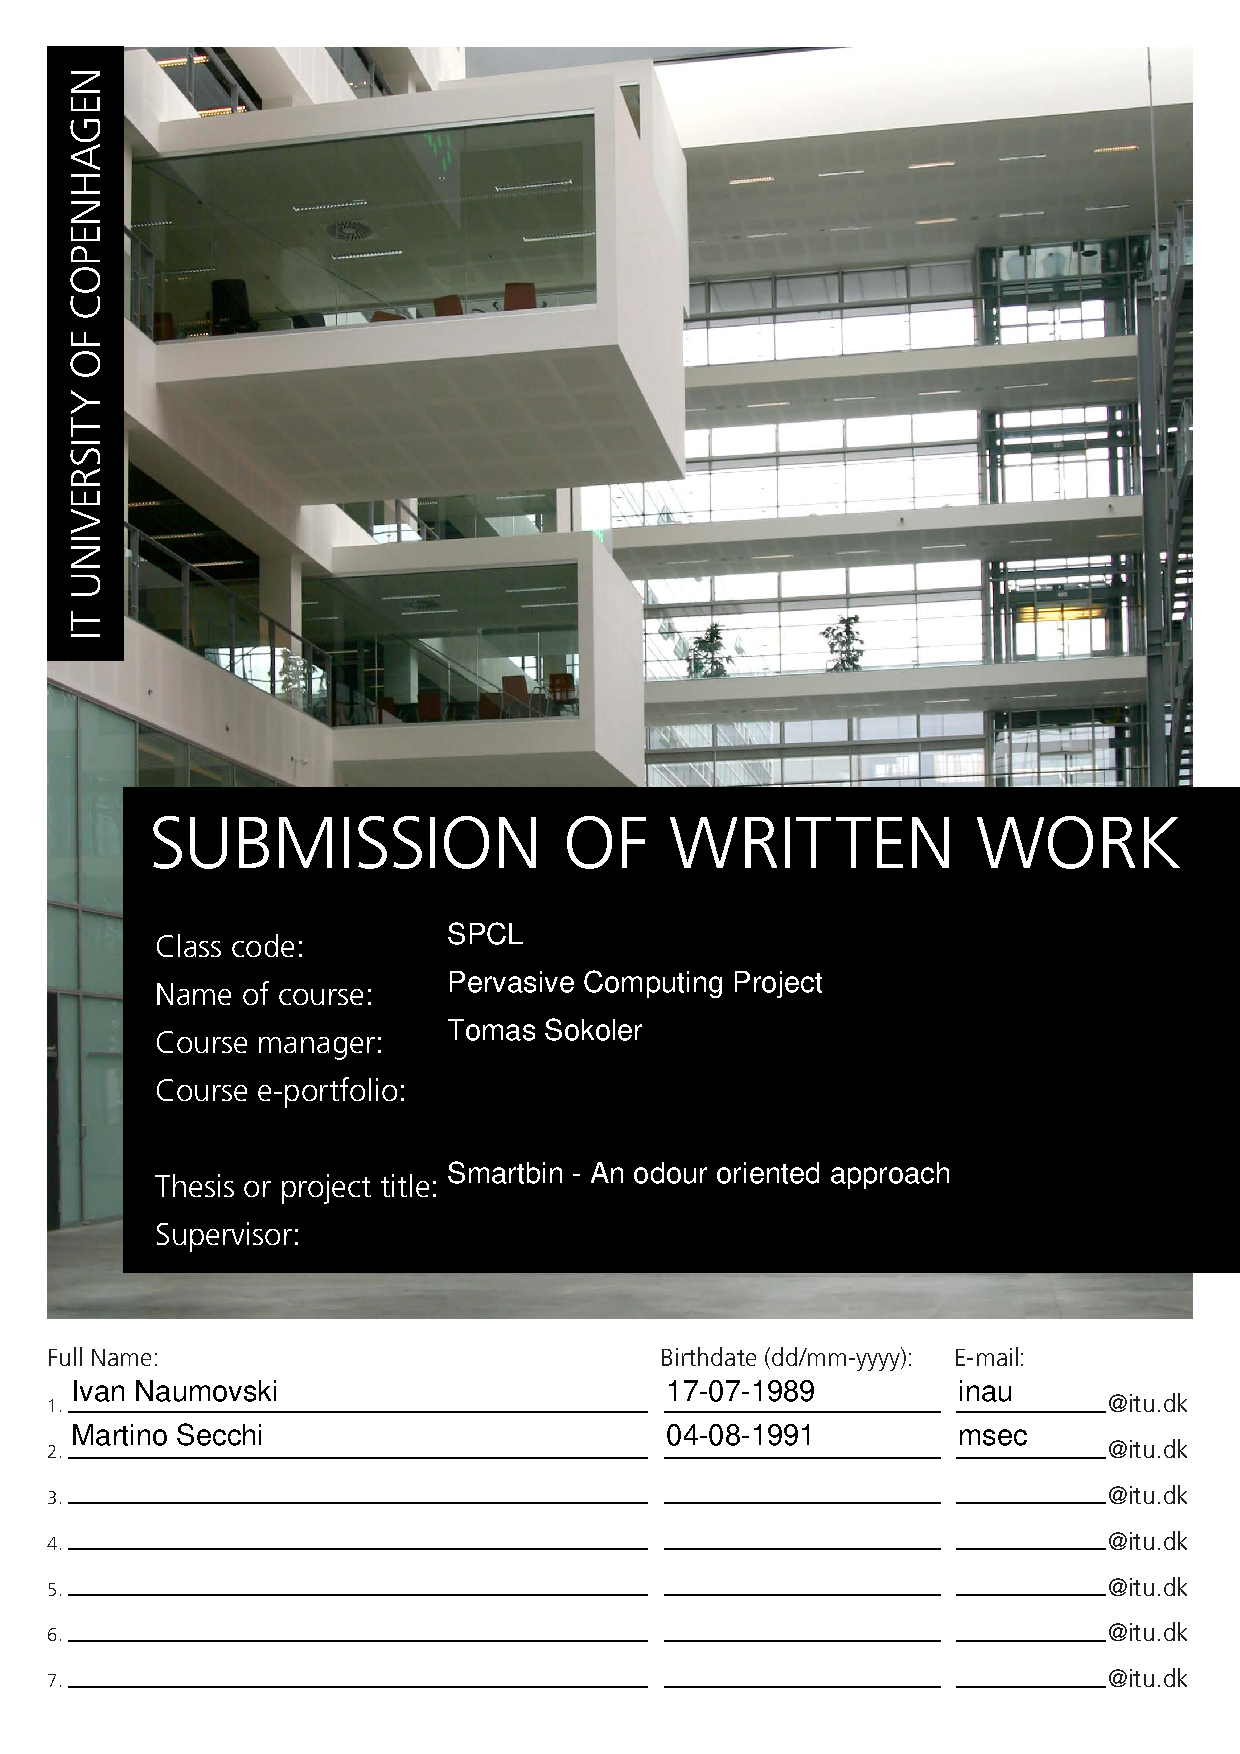
\includepdf{img/itu_front}
\pagenumbering{arabic}
\title{Smart Bin - An Odor Oriented Approach to Waste Management}

\numberofauthors{2}
\author{
  \alignauthor Ivan Naumovski\\
    \email{inau@itu.dk}\\
  \alignauthor Martino Secchi\\
    \email{msec@itu.dk}\\
}

\maketitle

\begin{abstract}
Technology enhanced trash cans have already been subject to research and have become available as market products.
How we handle the waste has traditionally been a logistics issue, but it can be approached also in other ways. \\
The SmartBin perceives the trash as something more than a pile of waste - it is also something smelly!\\
The emphasis is on improving the indoor environment to ultimately improve the quality of life by detecting odors.
The technology enhancing the bin uses sensors which detect gas emissions, mainly the ones occuring in decomposition of organic materials.
If any of these values exceed the threshold the SmartBin will react accordingly, supported by state of the art machine learning techniques \todo{nope}.
Any specifics will be listed in the following document. This will range from hardware prototyping to evaluation of the product.
\end{abstract}

\category{H.5.m.}{Pervasive computing, smart measuring}{Miscellaneous}
\category{C.2.4.}{Distributed systems}{Client/Server}
\category{C.3.}{Special-Purpose and Application-Based Systems}{Real-time and embedded systems}

\terms{
	Design; Measurement; Embedded devices; Internet of Things. 
}

\section{Introduction}
Waste management is a constant issue, that is dealt with on the daily by different organisations.
According to Eurostat, the countries in europe have had a rather stable production, while some countries fluctuate towards higher productions of waste other countries produce less.
The above supports the claim that waste management is highly relevant in a post modern society.

However waste management has been traditionally perceived from a logistical point of view.
Imagine not the amounts nor the location of the bin being the driving force for picking it up, but rather its smell.
This is the essential feature of our system - the additional parameter, which can be used in conjunction with existing systems or used to produce entirely new experiences centered around the waste bin.

\section{Related Work}
Smart Waste Management Systems (WMS) have been subject to extended research throughout the years.
The usual approach for data collecting in this area is to explore the physical attributes of a bin, namely what is put in the bin.
The common ways of obtaining such information are divided in two main categories: physical sensing and tagging.

Physical sensing is a great way to obtain generic information about the amount of garbage, and is usually measured in weight or height.
In recent years though, the use of tagging has become fairly popular, and some research in WMS has been conducted through the use of RFID tags and other tagging technologies.

With different technologies, in general come also different purposes.
While both approaches can handle well general monitoring and analysis of the processes revolving around waste management, some are better suited for specific uses.

Tagging technologies are excellent ways of tracking every object and associate meta information to them, therefore are often used in conjunction with recycling systems.
On the other hand, amount information is often used for systems that focus on resource allocation, garbage collection or process planning.

Systems with mixed approaches have also been developed.
%This information is traditionally used to perform advanced planning for collection of waste, or influencing people to adjust their behaviour in regards to what to throw out.

There are numerous examples of research in this area, we mention just few examples in the following paragraphs.

In a study conducted in Australia, a research group implemented an RFID and weight based system for real time automated WMS, with the main focus on bringing down management costs and facilitate automating waste identification~\cite{australia}.
In France, an RFID based system is instead focused in assisting in the recycling process by making sure that the waste is disposed correctly\cite{france}.

In another study performed in South Korea, the main approach was to analyse and identify food waste in a selected area of Seoul, and give citizens incentive to waste less food by fining them based on the amounts of waste they dispose~\cite{korea}. The distinction of trash was done using RFID, and the amount was measured in weight.

In an italian study, a Smart-M3 Platform and sensor enhanced bins were used, this was done with the main focus on urban planning, smart collection and  monitoring of urban solid waste \cite{catania}.\\
In this case, the information that was collected was on the location of the trash can, level of fullness, and weight of the waste.


It's worth mentioning that all of the previous examples don't account for gas emission or smell, even though some steps in this direction have been taken.
A research at MIT (Massachusetts Institute of Technology) enabled a trash can with a perfume dispenser, that would activate whenever gas emissions are detected from the trash\cite{perfume}.


%The infrastructure used in the variety of systems tends to be similar.
%Usual approach is a centralized server and a host of devices providing data to the server.\\
%The server is then used as a data provider for powering applications such as management utilities or phone apps.

\section{System Design}
Our approach includes the additional parameter of scent as a factor.
Biology supports our claim due to the fact that some materials are decomposed over time.
This decomposition has side effects, namely the production of certain gasses,
which can be detected by a variety of sensors due to their multiple characteristics of density and conductivity.
%Gasses can have multiple characteristics - hence a variety of sensors able to detect gasses exist.
We are interested in the gasses easily detectable by humans - namely the ones with a characteristic smell.
%Humans have a hard time detecting the odour-less ones.

Our system is composed of four main components, a \textit{sensory layer}, a \textit{communication module},  a \textit{	data layer}, and a \textit{data consumer}. 
%\begin{itemize}
%\item sensory layer: responsible of producing information, placed directly on the bin.
%\item communication module: responsible of sending such information.
%\item data layer (the cloud): this component stores the data and makes it available.
%\item data consumer (android):  this client shows information to the end user on request
%\end{itemize}

\subsection{Sensory layer and Communication module}
The sensory layer has two sensors (figure \ref{fig:sensors}) and one communication device. The sensors detect the state of the bin.
Our approach relies on two kinds of information related to the state of the bin: smell and fill level.
For this reason, the sensory part of the system is of key importance, since it enables the information to be perceived and registered by the system.
An odor detection sensor is able to capture volatile organic compounds (VOCs) and other gases, typical by products of food decomposition, commonly associated with bad smell. 
Some examples are Hydrogen Sulphide (\ce{H_{2}S}), Ammonia(\ce{NH_3}), Toluene (\ce{CH_3}) and others.
The smartbin sends the raw values of VOC concentration to the data layer.

The other type of sensor is a ultrasonic distance measurement unit. This is used to get the distance to the bottom of the bin.
This type of information is processed in the sensory layer to reflect the amount of thrash filled in the bin.

The raw values are then processed and formatted into something understandable for our data layer.
The last step is to send the values using the communication module. In this study a WiFi adapter was used.

\begin{figure}
\centering
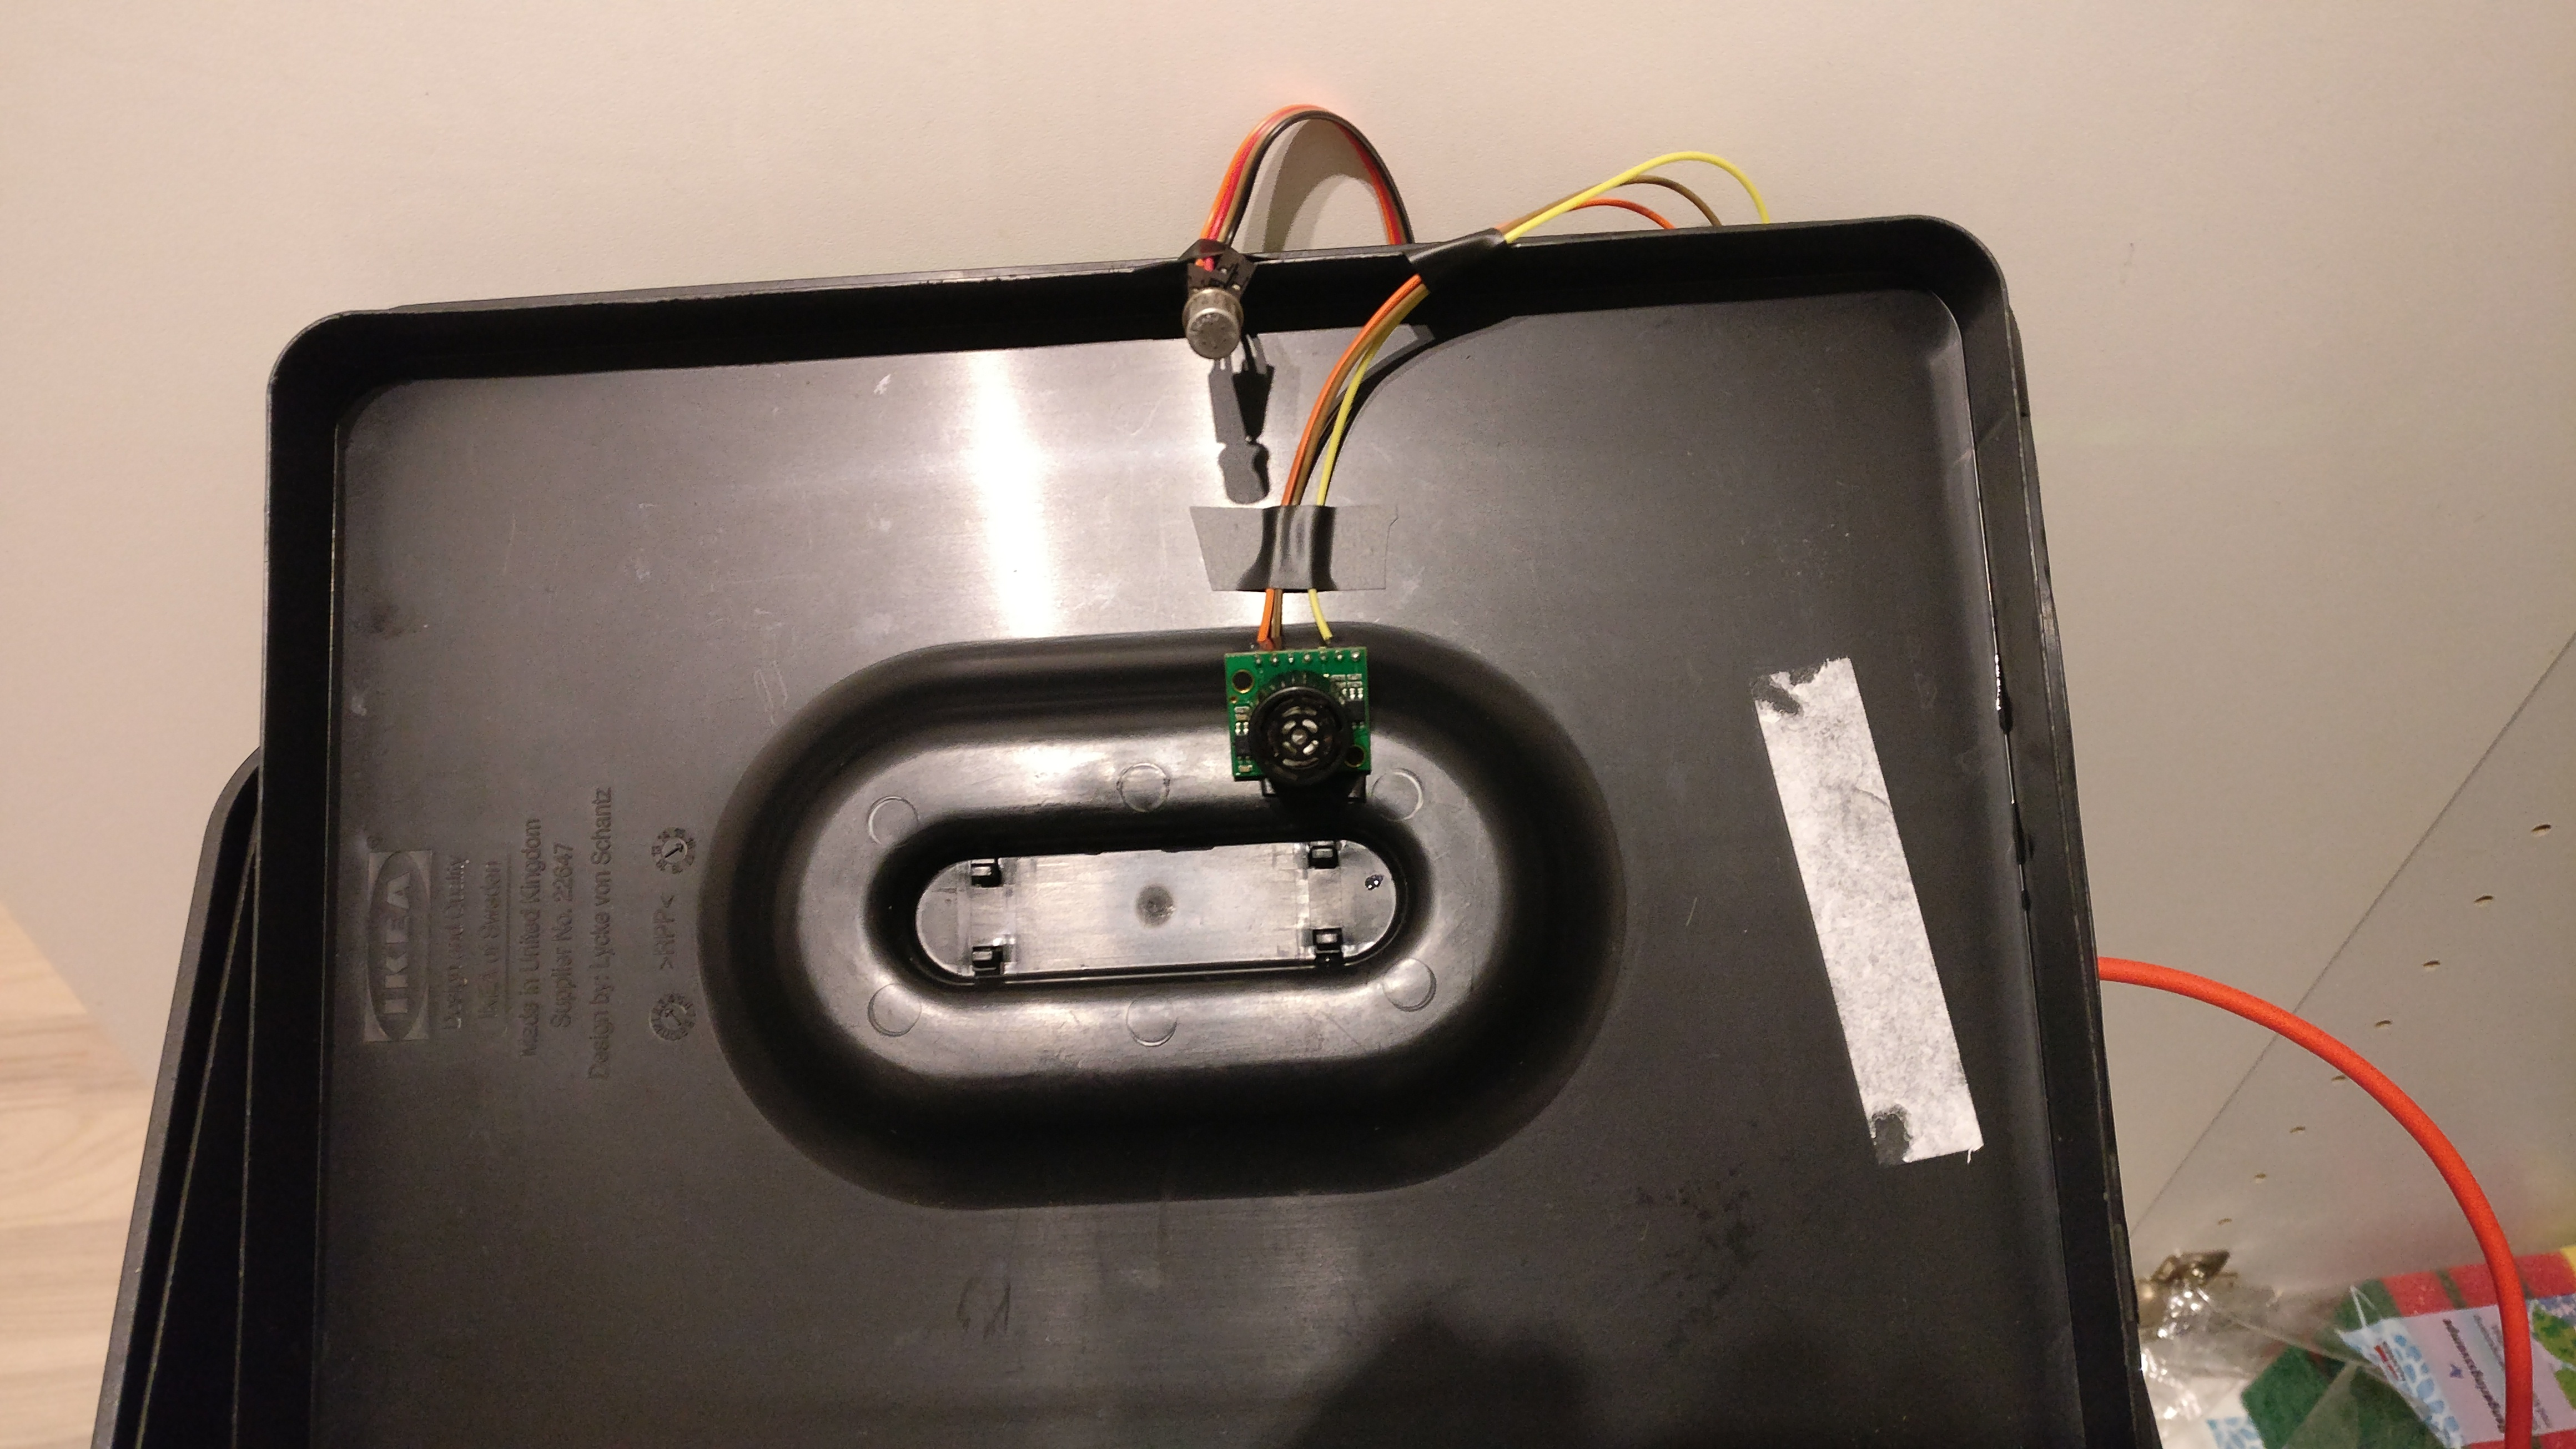
\includegraphics[scale=.05]{img/IMG_20161130_163302}
\caption{The sensors.}
\label{fig:sensors}
\end{figure}

\subsection{Data layer}
The data layer is a simple restfull webservice for collecting the data and storing it in a database, making it accessible to potential consumers.
The service supports two types of entities. The SmartBins and the contexts.
In short a SmartBin represents the hardware instance of a smartbin, this includes information such as location expressed as coordinates, unique identifier, 'calibration' which is the intial air quality level (in "clean" air, a value to which compare later measurements) and meta information about the last associated context.
This ensures that status of every bin is readily available without having to traverse the contexts.
The contexts model a snapshot of a bins state at a given time.

\subsection{Data Consumer}
The consumer in our case is an android client, but could just as easily have been any other platform able to connect to the internet and present content.

Our client can work in two separate modes: either as an android application or simply as an ambient display(single bin mode).

On the android application it is possible to manage multiple bins and get an overview of the last values measured by the system.

The ambient display is much more simple, it just displays a color of a shade from blue to red depending on the scent level.

In our system we use an android phone to run in both modes, so pressing on the screen even in ambient display mode will give the user the extra functionality of knowing trash level and emission level.

Ideally the ambient display can be placed in a strategic location inside the house, for example by the door or on the fridge, where people can be reminded of the trash status and act accordingly.

Figure \ref{fig:interaction} shows an example of interaction with the ambient display.

\begin{figure}
\centering
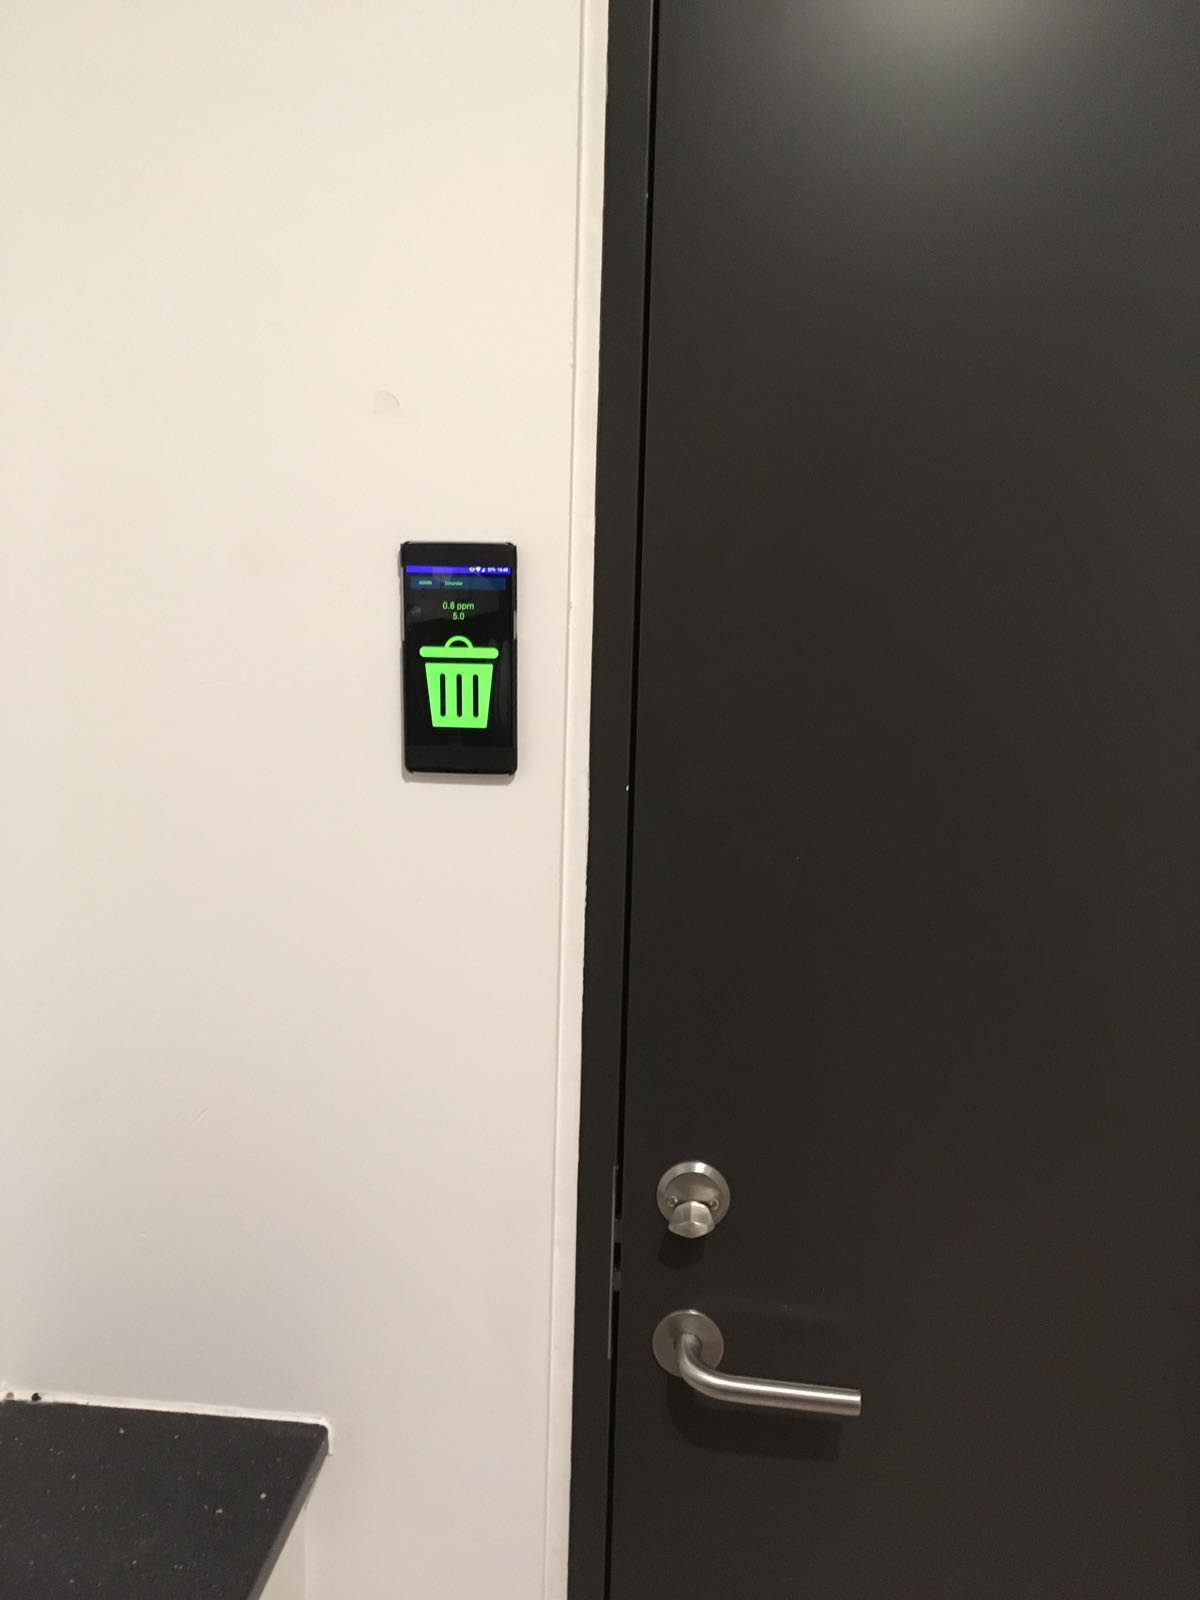
\includegraphics[scale=.05]{img/IMG-20161130-WA0000}
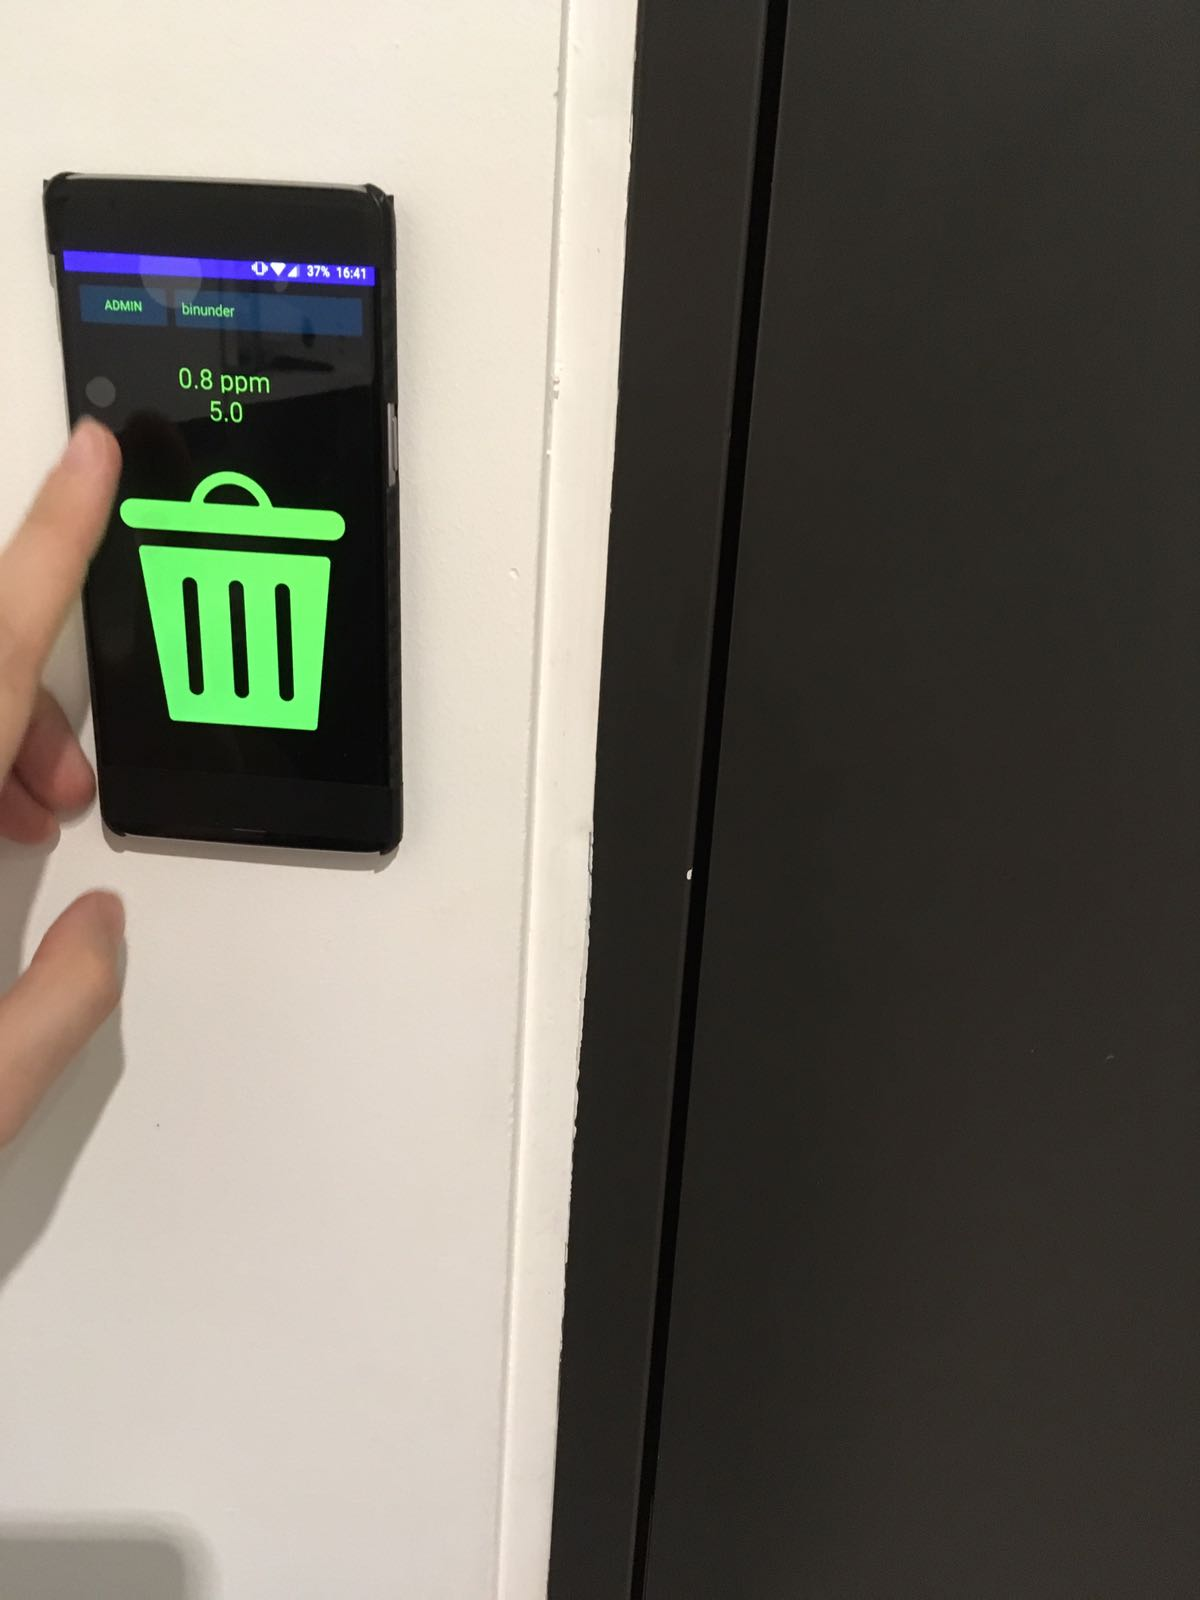
\includegraphics[scale=.05]{img/IMG-20161130-WA0004}
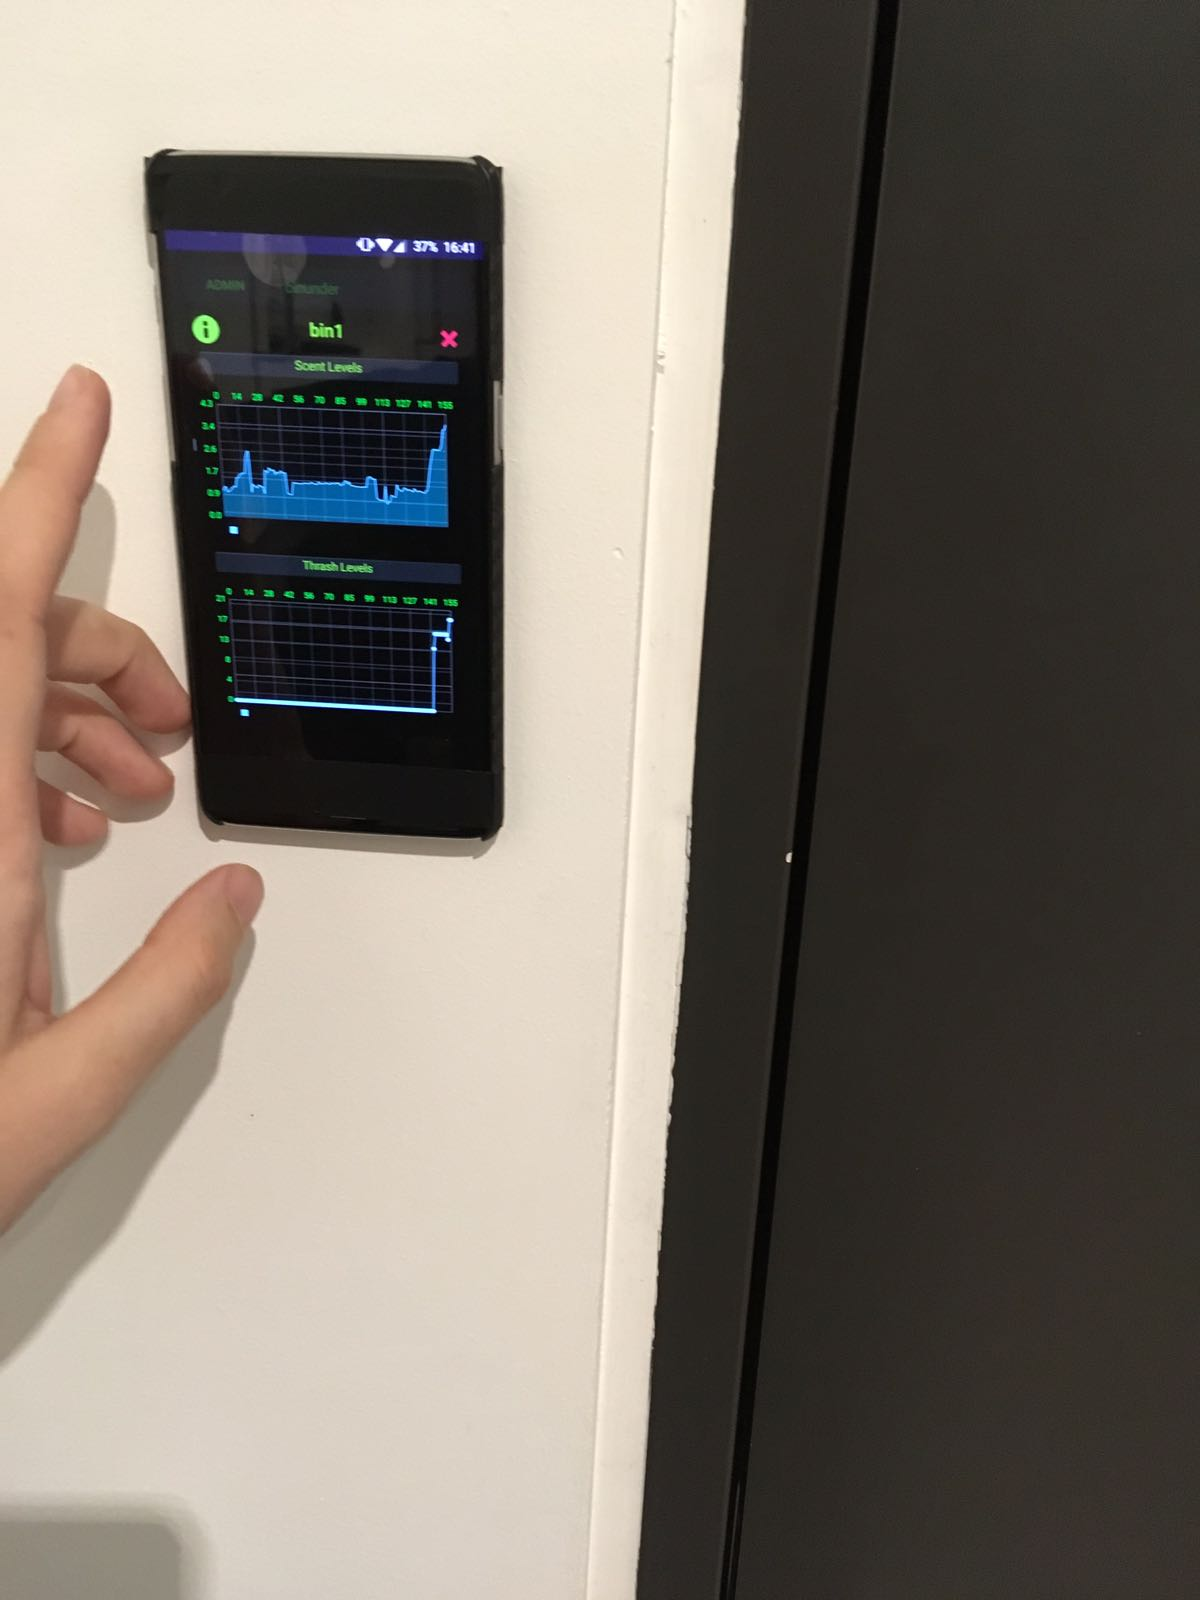
\includegraphics[scale=.05]{img/IMG-20161130-WA0002}
\caption{Interaction with ambient display}
\label{fig:interaction}
\end{figure}

\section{Hardware}
The Smartbin hardware platform is a simple construction consisting of two sensors, a microprocessor and a wifi communication module. It is embedded into a thrashbin with a lid which is used
as a base for both the distance sensor and the gas sensor.

We built the prototype using an Arduino Uno board.
 As for the sensors we used a Figaro TGS2602 as our gas sensor and a MaxSonar MB1013 ultrasonic rangefinder as our distance sensor.
We use a WiFi shield on the Arduino board for wireless communication.

The presentation layer works on Android 4.0 or later.

\section{Software}
\todo{todo}
to mention:
google app engine
android stuff, api for graphs, others?
arduino code detail?


\section{Evaluation}
The SmartBin system which has been constructed utilizes gas sensors to open up an additional dimension when measuring the state of the environment, in which it has been placed.

This extra dimension provides values of various gas concentrations in the current environment.
In short these values will be used in an evaluation of how the current environment is doing in regards to air quality and potential safety hazards for individuals.

The expectation is that these results can be used to produce rather precise predictions about how smelly the air in the given environment is.

People have a notion about what smells, machines need to do these predictions based on values from sensors.

The assumption is that the gas emissions of some chemical reactions, namely the ones where decomposition of organic materials is happening, always produce some specific gasses as a product.
It is based on our knowledge of these different gasses and how they smell - we assume that hightened concentrations of some of these gas types result in worse quality air.


\subsection{System Evaluation}

We interviewed a restricted poll of people in regards to usability of our system in a private scenario, and the results are the following:
\todo{actual findings?}

Multiple groups were used.

Group A where a homogenous group of people, all males and all ranging between the age of 20-30.
They keep their thrash bin below their sinks in the kitchen, and some also have additional bins in the bathroom.
The bathroom bins were not deemed that relevant due to the fact that most bathrooms are subject to having smelly environments post use.

Interviews collecting the opinion of the group  were performed.
The procedure was to present images of the bin and let the participants play around with the android application, followed by a non-chalant conversation of the system.
All three people expressed that the system seemed like something obsolete. They were all really good at taking out the thrash.
And the idea of having a situated display on either the wall or the outside of the thrash cabinet was stupid due to the fact that one could just open up and see.

all of the interviewed keep their private trash under the sink in a closed compartment

most of the interviewed consistently forget to take out the trash when they should

most of the interviewed think a reminder on the trash status placed on the door would be extremely useful to remember to take the trash out

evrybody think it's cool

stuff


\section{Discussion}
\iffalse
discussion

here emphasize  about the famous What IF question

take this INNOVATIVE aspect and use it in waste management

in the conclusion:
we can build it, it works, the technology is out there
in the discussion:
it can be applied somewhere else
it can extend other systems
used for innovation
it's a different take
\fi

The SmartBin system which has been constructed utilises gas sensors to open up an additional dimension when measuring the status of the trash present in bins.
This extra dimension is the main focus of our system, as an innovative angle on an existing problem.

In this section we want to discuss some of the openings that this approach allows.

What if we could use this data to expand our take on waste management systems?
Logistic for garbage collection is usually driven by amounts, but what if bad smell was also one of the leading parameters to act upon?

Large levels of bad smell emitting from the trash result in unsanitary conditions, insalubrity and worst air quality, and attract insects and other wild animals.
While it remains true that trash handling is first and foremost a logistical issue, most waste management systems don't take bad smell into account at all.

By for example prioritising the collection of "smelly" garbage, alongside with the collection of full trash cans, insalubrity conditions might be reduced significantly.
This would ultimately improve air quality and the quality of life around public spaces.

 

\iffalse
%old evaluation
The SmartBin system which has been constructed utilises gas sensors to open up an additional dimension when measuring the state of the environment in which it has been placed.
This extra dimension provides values of various gas concentrations in the current environment.
In short these values will be used in an evaluation of how the current environment is doing in regards to air quality and potential insalubrity hazards for individuals.
The expectation is that these results can be used to produce rather precise predictions about how smelly the air in the given environment is.
People have a notion about what smells, machines need to do these predictions based on values from sensors.
The assumption is that the gas emissions of some chemical reactions, namely the ones where decomposition of organic materials is happening, always produce some specific gases as a product.
It is based on our knowledge of these different gasses and how they smell - we assume that hightened concentrations of some of these gas types result in worse quality air.


%old conclusion
While it remains true that trash handling is first and foremost a logistical issue, most waste management systems don't take bad smell into account.
Our claim is that bad smell is actually a part of the problem when talking about trash management,  both in the private as well as in the public.

While a private IoT "smart bin" that includes smell information would serve the ultimate goal of assisting in the process of garbage collection, it can be extended also for other purposes like data collection or as a perfume dispenser \cite{perfume}.
On the other hand, when approaching waste management from a urban point of view, the focus is often placed on the logistics: urban planning (where to place the bins, how many, ..) and on route planning for garbage collection.
These systems usually rely on information on amounts of trash, being it height values or weight.
Our claim \todo{not supported by proof} is that smell information could also be relevant.
\todo{rephrase or change, too tired right now}
\fi

\section{Conclusion}
The system described above is a simple implementation of what a private waste management system can look like. 
With the right IoT components, trash status can be easily monitored and transmitted.
Modern sensors allow machines to perceive the same as what humans can, if not more at times, making it possible to even detect bad smell in our trash.
Here is where our system separates itself from most of the other products in the same area.
This extra parameter could be exploited to potentially be one of the leading information considered in waste management, together with the more canonical weight and amount. 

While it remains true that trash handling is first and foremost a logistical issue, most waste management systems don't take bad smell into account.
Our claim is that bad smell is actually a part of the problem when talking about trash management,  both in the private as well as in the public.

While a private IoT "smart bin" that includes smell information would serve the ultimate goal of assisting in the process of garbage collection, it can be extended also for other purposes like data collection or as a perfume dispenser \cite{perfume}.
On the other hand, when approaching waste management from a urban point of view, the focus is often placed on the logistics: urban planning (where to place the bins, how many, ..) and on route planning for garbage collection.
These systems usually rely on information on amounts of trash, being it height values or weight.
Our claim \todo{not supported by proof} is that smell information could also be relevant.
\todo{rephrase or change, too tired right now}

\bibliographystyle{acm-sigchi}
\bibliography{report}
\end{document}
